\documentclass[14pt,a4paper,oneside]{article}

\usepackage[utf8]{inputenc}   


\usepackage{amsmath,amsthm,amssymb,appendix,bm,mathrsfs,ctex,geometry,tcolorbox,fancyhdr,tikz,esint,appendix}


%% GB/T 7714 宏包 ---- 引文格式
\usepackage[sort&compress]{gbt7714}
\bibliographystyle{gbt7714-numerical}



\numberwithin{equation}{subsection}             %%%%%% 公式编号




\geometry{left=1.7cm, right=1.7cm, top=2.54cm, bottom=2.54cm}    %%%%% 页面尺寸
\linespread{1.5}                             %%%%% 行距1.5倍
\pagestyle{fancy}



%%    设置页眉页脚
\fancyhf{}
\renewcommand{\headrulewidth}{0.15mm}
\fancyhead[C]{文献阅读报告}                   %%%%%% 页眉
\fancyfoot[C]{\thepage}                      %%%%%% 页脚 页码
\setlength{\headheight}{15pt}


%%   设置各种链接颜色为黑色
\usepackage[colorlinks,
            linkcolor=black,
            anchorcolor=black,
            citecolor=black,
            urlcolor=black
            ]{hyperref}



%%   例子编号
\newcounter{example}
\counterwithin{example}{subsection}
\newcommand{\examplename}{Example}
\newcommand{\exampleTitle}[1]{%
\textbf{\refstepcounter{example}\examplename\theexample:#1}\par}


%%  插入图片配置
\usepackage{graphicx,subfigure}
\usepackage[]{caption2} %新增调用的宏包
\numberwithin{figure}{subsection}               %%%%%% 图片编号

\graphicspath{ {./Figure/} }            %%%%% 设置图片文件所在目录
\DeclareGraphicsExtensions{.pdf,.svg,.jpeg,.png,.jpg}     %%%%% 支持图片格式


%%    支持tikz作图
\usepackage{tikz}
\usetikzlibrary{backgrounds,arrows}


\usepackage{pgfplots}
\pgfplotsset{compat=1.15}
\usepackage{mathrsfs}


\title{\textbf{文献阅读报告 7\\Ultrafast nonlinear optics in gas-filled hollow-core photonic crystal fibers [Invited]}}                           %%%%% 标题
\author{骆禹天}                                           %%%%% 作者
\date{2024/**/**}                                        %%%%%% 日期

%%   定义一些数学格式
\newtheorem{theorem}{定理}[subsection]
\newtheorem{definition}[theorem]{定义}
\newtheorem{lemma}[theorem]{引理}
\newtheorem{corollary}[theorem]{推论}
\newtheorem{example}[theorem]{例}
\newtheorem{proposition}[theorem]{命题}
\renewcommand{\abstractname}{\Large\textbf{摘要}}




%------------------------- 开始文档  -------------------------%



\begin{document}

\pagenumbering{Roman}         %%%%% 目录前页码统计按罗马数字

\maketitle

\setcounter{page}{1}          %%%%% 标题开始统计页数

%------------------------- 目录  ------------------------------%

\tableofcontents              %%%%% 插入目录

\newpage
\setcounter{page}{1}          %%%%% 目录后重新统计页数


\pagenumbering{arabic}        %%%%% 目录后统计页码为阿拉伯数字



%%%%%%%%%%%%%%%%%%%% 开始第一节  %%%%%%%%%%%%%%%%%%%%%



\section{Introduction}



固体芯光纤 (Solid-core fiber, 传统或光子晶体) 优势:

· 超长的有效路径长度

· 一致和可预测的色散

· 可配置的双折射

· 非线性优值 (非线性和损耗之间的平衡) , 对于二氧化硅光纤来说, 这是所有介质中最高的. 

应用:

· 光孤子的观测, 孤子自频移的发现, 

· 超快全光开关的发展, 

· 跨倍频程超连续谱

· 连续波泵浦超连续谱的产生, 

· 四波混频、

· 调制不稳定性 (MI),

· 自相位调制,

· 拉曼和布里渊散射,

· 自组织二次谐波产生.

固体光纤问题: 由于基于全内反射, 传统光纤纤芯折射率必须高于包层折射率, 因而无法将非线性光纤拓展到气体和等离子体芯 (气体折射率接近1——光学频率下低于任何电介质材料). 

气体使用必要情况, 如在展宽毫焦量级持续时间为飞秒量级的800 nm脉冲光谱时, 要避免光学损伤. 玻璃毛细管提供了部分解决方案, 尽管不支持束缚模, 但$\mathrm{HE_{11}}$泄漏模式的损耗与孔径的倒数成正比, 在800 nm波长下, 直径为$\sim$ 200 $\mathrm{\mu m}$时, 损耗低至 1.2 dB/m. 即使这种尺寸的孔径中支持许多更高阶的泄漏模式, 但如果仔细调节, 也有可能仅激发$\mathrm{HE_{11}}$模式. 

气态纤芯另一吸引人的特点是可通过改变气压调节非线性和群速度色散 (GVD) . 大口径真空毛细管中 $\mathrm{HE_{11}}$ 模的 GVD 很弱, 而惰性气体 GVD 在光频率下是正常色散. 然而, 事实证明, 在比较有用的气压下, 充气毛细管中的零色散点往往远移至红外 (IR) 区域, 且总体 GVD 在紫外 (UV) 至近红外 (NIR) 光谱范围都几乎是正常色散区域, 这极大地限制了可实现的超快非线性动力学的范围. 

HC-PCF \cite{creganSingleModePhotonicBand1999, counyLargepitchKagomestructuredHollowcore2006, stjrussellPhotoniccrystalFibers2006, russellPhotonicCrystalFibers2003, knightPhotonicCrystalFibres2003}克服了这些限制, 提供超长单模相互作用长度 ($\sim$ 10 甚至$\sim$ 1000 m) 、每瓦特功率有高的强度 (由于纤芯直径小) 、高光学损伤阈值并且支持精细的 GVD 控制. 这些已被广泛应用于各种实验中\cite{bhagwatNonlinearOpticsHollowcore2008, benabidLinearNonlinearOptical2011}, 如展示了受激拉曼散射中孤立波和自相似性\cite{abdolvandSolitaryPulseGeneration2009, nazarkinDirectObservationSelfsimilarity2010}、进行良好控制的相干原子物理实验\cite{londeroUltralowpowerFourwaveMixing2009, ghoshResonantOpticalInteractions2005}、传递高强度能量的光学孤子\cite{ouzounovGenerationMegawattOptical2003}和粒子引导\cite{benabidParticleLevitationGuidance2002}. 

\section{HC-PCF 的特性}

HC-PCF 主要有两类\cite{creganSingleModePhotonicBand1999, counyLargepitchKagomestructuredHollowcore2006, stjrussellPhotoniccrystalFibers2006, russellPhotonicCrystalFibers2003, knightPhotonicCrystalFibres2003}. 

第一种, 基于全二维光子带隙 (称为 PBG 引导 HC-PCF来限制光) , 最常见的结构由气孔组成的六边形网格组成, 如图\ref{p2.0.1}所示. 

\begin{figure}[h]
    \centering
    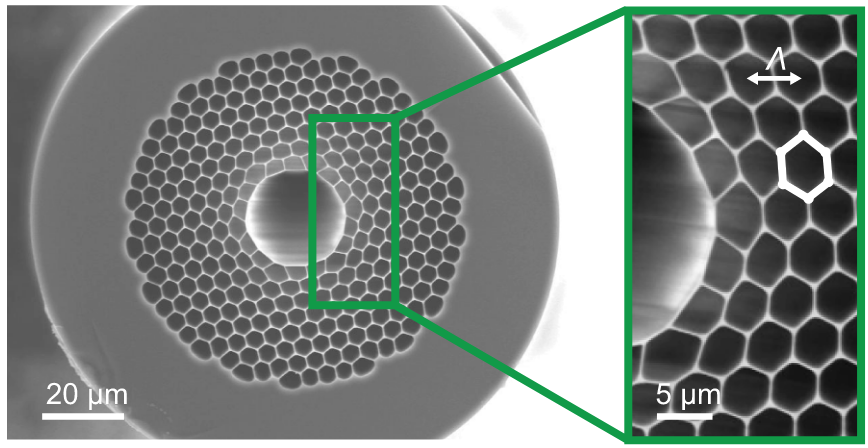
\includegraphics[width=0.3\textwidth]{p1.png}
    \caption{PBG 引导 HC-PCF 的 SEM}\label{p2.0.1}
\end{figure}

其可提供极低的传输损耗 (最好情形在 1550 nm 损耗 <1 dB/km) \cite{robertsUltimateLowLoss2005}, 在有限的光谱范围内引导严格限制的单模. 此功能对于光谱过滤非常有用, 例如, 可以抑制拉曼散射中不需要的斯托克斯频带\cite{benabidUltrahighEfficiencyLaser2004}. PBG 引导 HC-PCF 的 GVD 具有陡峭的斜率, 在传输窗口内通过零并在其边缘获得非常大的值. 为了说明这一点, 图 \ref{p2.0.2} 显示了设计在 800 nm 下工作的理想结构的有限元建模 (FEM) 计算结果. 

\begin{figure}[h]
    \centering
    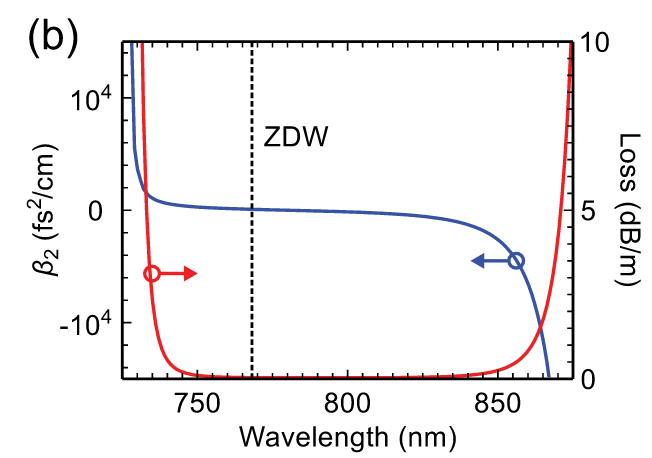
\includegraphics[width=0.3\textwidth]{p2.png}
    \caption{理想 PBG 引导 HC-PCF 结构的 FEM 计算 GVD 和损耗, 该结构设计用于在 800 nm 左右运行, 芯直径 11 $\mathrm{\mu m}$, 节距 ($\Lambda$) 2.1 $\mathrm{\mu m}$}\label{p2.0.2}
\end{figure}

在 800 nm 附近计算损耗为 0.01 dB/m. 零色散波长 ZDW 位于 768 nm, 色散在窄传输带上变化很大, 在零色散点色散斜率大于 2000 $\mathrm{fs^3/cm}$. PBG 引导 HC-PCF优点是极低的损耗使这些光纤可用于广泛的应用, 但缺点是有限的传输窗口和极端的色散斜率阻碍了其应用于极端超快脉冲实验. 

第二种类型 HC-PCF 基于 kagomé 晶格包层, 形成大卫之星图案的玻璃网络, 如图 \ref{p2.0.3} (c) 所示. 

\begin{figure}[h]
    \centering
    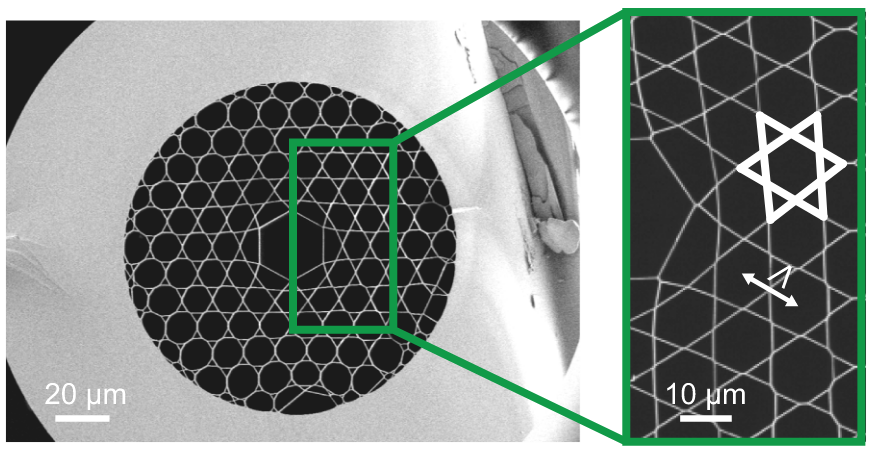
\includegraphics[width=0.3\textwidth]{p3.png}
    \caption{Kagomé PCF 的 SEM 图像, 为在 UV 和 800 nm 左右范围工作而设计}\label{p2.0.3}
\end{figure}

它以 $\sim$1 dB/m 的损耗水平提供超宽带 (几百纳米) 传导, 并在整个传输窗口上呈微弱的反常 GVD (排空时, $|\beta_{2}| < 15\;\mathrm{fs^{2}/cm}$), 色散斜率较低. 

图 \ref{p2.0.4}为一种示例结构 (30 $\mathrm{\mu m}$ 芯直径, 设计用于在 UV 和 800 nm 左右工作) 的 FEM 计算, 展现了宽带引导窗口 (200-350 nm 和600-850 nm 处 < 2 dB/m), 并在整个频带内具有相对较小的全反常色散 (低于 15 $\mathrm{fs^{2}/cm}$). 

\begin{figure}[h]
    \centering
    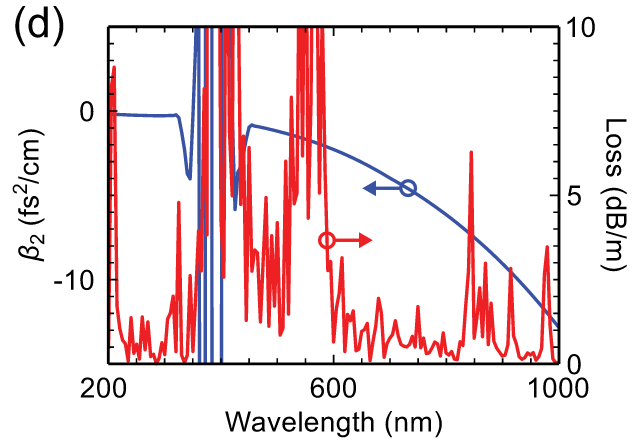
\includegraphics[width=0.3\textwidth]{p4.png}
    \caption{使用理想 kagomé PCF 结构的 FEM 计算 GVD 和损耗, 该结构具有 30 $\mathrm{\mu m}$ 芯直径、15 $\mathrm{\mu m}$ 节距 ($\Lambda$) 和 0.23 $\mathrm{\mu m}$ 网格厚度. }\label{p2.0.4}
\end{figure}

这不包函在 $\sim$ 380 nm 处具有反交叉伴随强烈的包层共振, 这种包层共振会破坏传输窗口, 但通常非常窄, 因此对全局色散特性影响很小. 此外, 还可通过改变网格厚度从而调整其远离特定应用所需波长带. 

与毛细管纤维不同, 惰性气体正常 GVD 可以与 kagomé PCF 的异常 GVD 相平衡, 从而只需改变气压便能实现 ZDW 在 UV、可见光和 NIR 光谱区域内进行调谐, 这使得该系统非常适合超快应用.

\subsection{充气 Kagomé HC-PCF 的色散和损失}

Kagomé HC-PCF 的模态折射率非常接近于毛细管纤维的模态折射率
\begin{equation}
    n_{mn}(\lambda,p,T)=\sqrt{n_{\mathrm{gas}}^2(\lambda,p,T)-\frac{u_{mn}^2}{k^2a^2}}\simeq1+\delta(\lambda)\frac p{2p_0}\frac{T_0}T-\frac{u_{mn}^2}{2k^2a^2}
    \label{eq:2.1.1}
\end{equation}
其中 k 是真空波矢, $n_{\mathrm{gas} }$ 是填充气体的折射率, $\delta(\lambda)$ 是 $n_{\mathrm{gas}^{2} }$的 Sellmeier 展开式, p 是压力, $p_{0}$ 是大气压力, T 是温度, $T_{0}= 273.15 \mathrm{K} $, $u_{mn}$ 是第一类 m 阶贝塞尔函数的第 n 个零点, 其中 $m=n=1$ 对应于光纤的 $\mathrm{HE_{11}}$ 模. 

可以为用于近似方程 1 中的 Kagomé 光纤芯的圆定义几个芯半径 a, 一个保留核心面积 ($a_{A}$), 另一个基于六角形核心的平面到平面距离 ($a_{f}$ ) , 如图 2(a) 的插图所示. 

\begin{figure}[h]
    \centering
    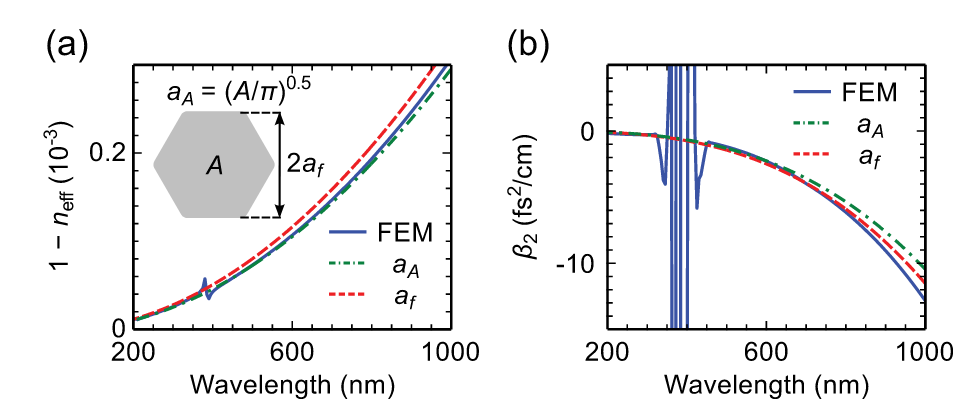
\includegraphics[width=0.4\textwidth]{p5.png}
    \caption{FEM 和毛细管模型之间的比较：(a) 有效模式指数的离散度和 (b) GVD.  (a) 插图, 两个核心半径的定义：平面到平面半径 ($a_{f}$ ) 和面积保留半径 ($a_{A}$)； A为六边形核心面积.  FEM 结果中 $\sim$ 380 nm 处的扭结由包层态的反交叉引起, 它强烈影响色散}\label{p2.1.1}
\end{figure}

与有限元模拟比较, 方程 \ref{eq:2.1.1} 近似十分贴近[图\ref{p2.1.1}(a) 和 (b)], $a_{A}$ 在比较有效模式指数时提供最佳一致性, 而 $a_{f}$ 在 GVD 计算时提供了最佳一致性.  \ref{eq:2.1.1} 的有效性已通过高阶导模中的相位匹配三次谐波生成得到进一步证实\cite{noldPressurecontrolledPhaseMatching2010}. 

kagomé PCF 色散特性与毛细管相似, 但损耗低得多. 对于$\sim$ 30 $\mathrm{\mu m}$的纤芯直径(在合理的非线性水平下是实现反常色散所需——见下文) , 毛细管中损耗超过几百 dB/m, 而 kagomé PCF损耗可低于 1 dB/m, 如图\ref{p2.1.2}. 

除了具有足够低损耗的宽带引导, 调节 kagomé PCF 内压力可以调节色散. 图 \ref{p2.1.2}(c) 显示了如何在整个紫外-可见光谱区域内调节填充 Ar 的 kagomé PCF(30 $\mathrm{\mu m}$ 芯直径) 的 ZDW, 例如允许在深紫外中形成孤子. 

\begin{figure}[h]
    \centering
    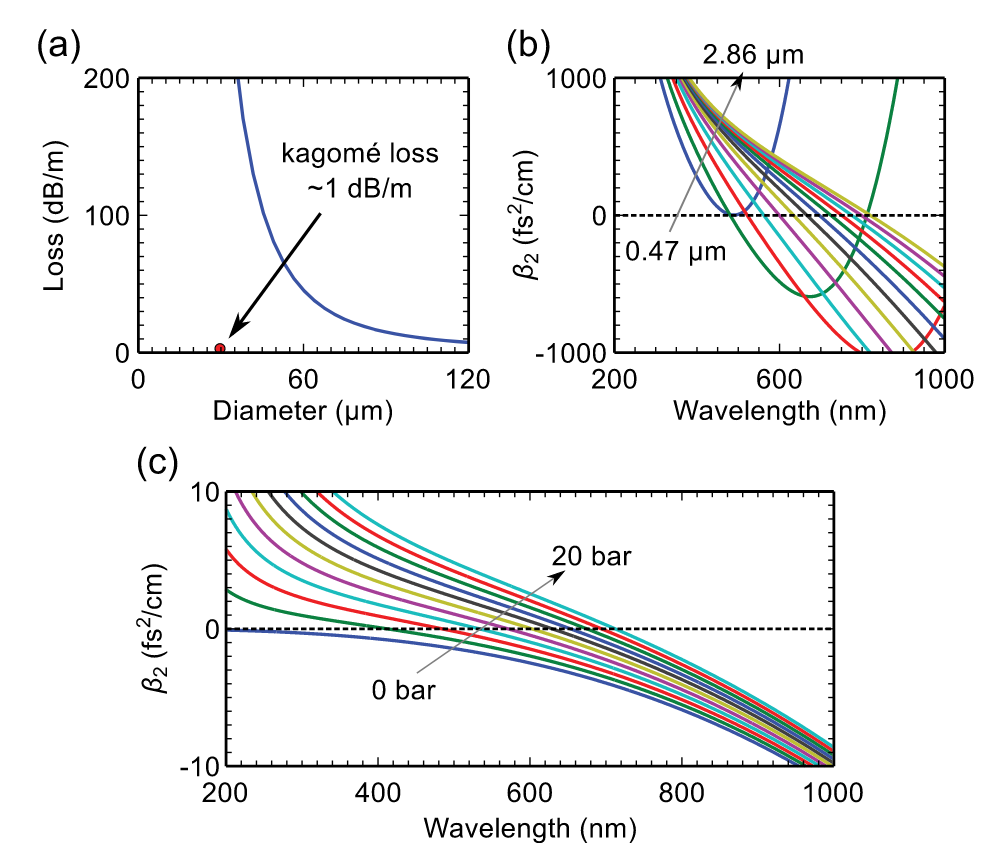
\includegraphics[width=0.4\textwidth]{p6.png}
    \caption{(a) 毛细管中最低理论损耗与芯直径为 30 $\mathrm{\mu m}$ 的 kagomé PCF 测量损耗间比较, (b) 具有最短的 ZDWs 的硅芯 PCF, 芯直径为 0.47 至 2:86 $\mathrm{\mu m}$(0.2 $\mathrm{\mu m}$ 步长), (c) kagomé PCF 的色散, 芯直径为 30 $\mathrm{\mu m}$, 填充有 0 至 20 bar Ar(2 bar) 步长) }\label{p2.1.2}
\end{figure}

这种特点与实心 PCF 比较很有趣. 尽管玻璃色散广泛而灵活, 但玻璃强烈的材料色散将最短 ZDW 限制为$\sim$ 500 nm [图 \ref{p2.1.2}(b)]. 实心 PCF 允许孤子在 800 nm 处传播并进入可见光区, 而 kagomé PCF 则在紫外区首先实现反常色散. 此外, kagomé PCF 色散幅度小得多, 即脉冲展宽速度慢得多, 离散频率的脉冲分离的速度要慢得多. 与实芯 PCF 相比, kagomé PCF有更长的非线性相互作用长度. 并且相对较小的色散斜率还意味着对孤子传播的扰动减少, 从而支持更短的自压缩脉冲生成. 

图 \ref{p2.1.3} 总结了改变气体类型、压力和纤芯直径调节 ZDW. 不仅可深入紫外区域, 还可以调谐至 1000 nm 以上的红外区域, 允许 800 nm 处的正常色散, 适用于下面讨论的光纤光栅/镜面压缩器等应用. 

\begin{figure}[h]
    \centering
    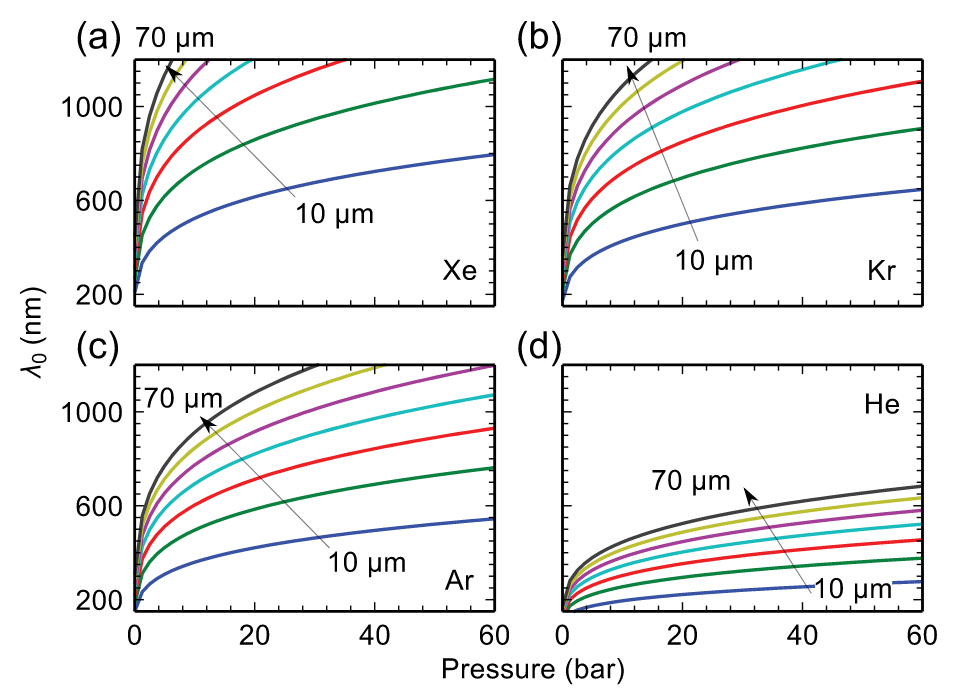
\includegraphics[width=0.4\textwidth]{p7.png}
    \caption{Kagomé PCF 的 ZDW, 直径为 10 至 70 $\mathrm{\mu m}$(步长为 10 $\mathrm{\mu m}$) , 填充有 0 至 60 bar 的 (a) Xe、(b) Kr、(c) Ar 和 (d) He}\label{p2.1.3}
\end{figure}

\subsection{充气 Kagomé PCF 的非线性}

假设基本 $\mathrm{HE_{11}}$ 模的模态强度分布形式为 $J_0^2(u_{11}r/a)$, r 为径向坐标, 有效模面积的传统定义得出 $A_{\mathrm{eff} }\approx1.5\;a^{2}$, 即, 芯直径为 30 $\mathrm{\mu m}$ 的 kagomé PCF 的 $A_{\mathrm{eff}}=338 \mathrm{\mu m}$. 实验和数值模型表明, 玻璃对 Kagomé PCF 非线性的贡献通常可以忽略不计, 因为玻璃中的光比例与包层谐振的距离小于 0.01\% [图\ref{p2.2.1}(a)]\cite{jolyBrightSpatiallyCoherent2011, lehmeierNonresonantThirdOrder1985}. 

\begin{figure}[h]
    \centering
    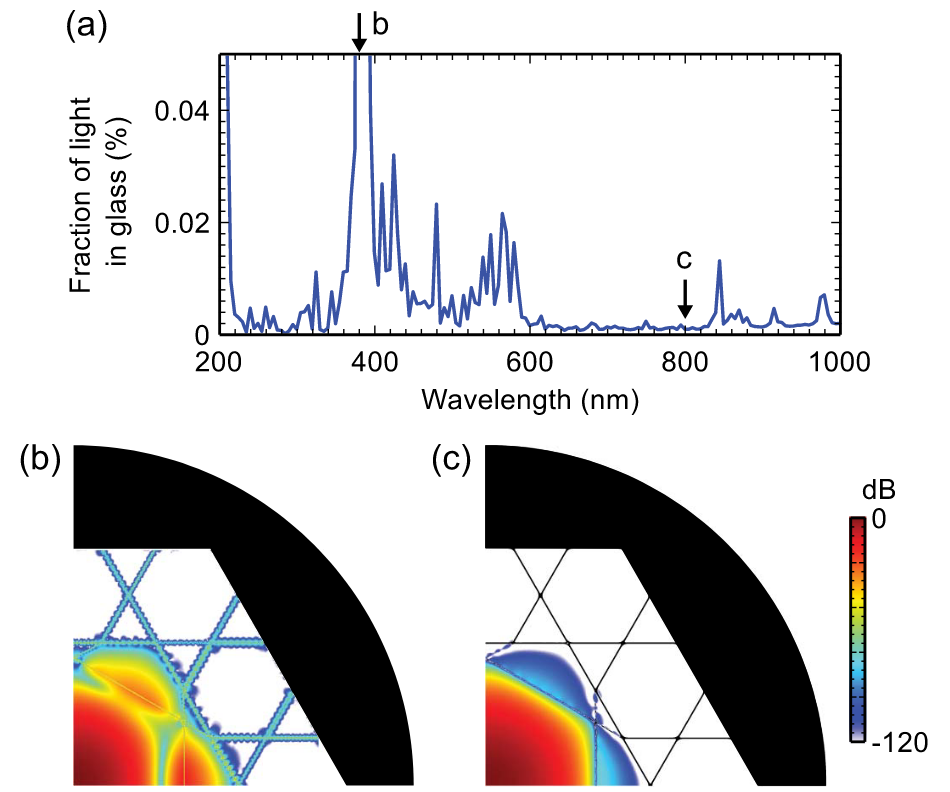
\includegraphics[width=0.4\textwidth]{p8.png}
    \caption{针对具有 30 $\mathrm{\mu m}$ 芯直径、15 $\mathrm{\mu m}$ 节距和 0:23 $\mathrm{\mu m}$ 腹板厚度的理想 kagomé PCF 进行的 FEM 计算 — 设计用于在 UV 和 800 nm 左右工作：(a) 功率分数的波长依赖性在玻璃中, (b) 包层谐振波长 (380 nm) 处传输模式坡印廷矢量的轴向分量, (c) 与 800 nm 处的 (b) 相同. }\label{p2.2.1}
\end{figure}

气体非线性与气体密度或恒温下压力成线性关系\cite{lehmeierNonresonantThirdOrder1985}. 对于芯直径为 30 $\mathrm{\mu m}$ 的 kagomé PCF, 非线性系数 $\gamma$ (在10 bar)为: 

$1.5 \times  10^{-7}\;\mathrm{m^{-1}W^{-1}}$ (Ne),
 
 $ 2 \times  10^{-6} \;\mathrm{m^{-1}W^{-1}}$ (Ar), 
 
 $ 5.3 \times  10^{-6} \;\mathrm{m^{-1}W^{-1}}$ (Kr),
 
 $ 1.5 \times  10^{-5} \;\mathrm{m^{-1}W^{-1}}$ (Xe). 
 
 这些比实芯 PCF 小 4 个数量级以上(芯直径为 1 $\mathrm{\mu m}$ 时为 $0.24\; \mathrm{m^{-1}W^{-1}}$) , 但比孔径为 200 $\mathrm{\mu m}$ 的充气毛细管高得多 $\sim 5 \times  10^{-8}\; \mathrm{m^{-1}W^{-1}}$ (10 bar Ar). 

Ar等单原子气体无拉曼散射, 可在无孤子自频移下研究孤子动力学和脉冲压缩. $\mathrm{N_{2}}$ 或 $\mathrm{SF_{6}}$ 等分子气体可在 kagomé PCF 中研究拉曼散射. 对于超快应用, 一种可能是将不同拉曼贡献气体混合, 引入比例连续可调的拉曼贡献. 

除微扰束缚电子非线性外, kagomé PCF 在微焦量级下足以电离气体产生部分等离子体. 尽管在 kagomé PCF 中的自由电子密度和光强度下, 场-等离子体相互作用通常线性, 但电子生成过程既超快又高度非线性, 导致新的非线性效应, 例如孤子自频率蓝移. 

\subsection{Kagomé HC-PCF 的能量处理能力}

玻璃中的功率的有限元计算如图 \ref{p2.2.1}(a) 所示, 在 800 nm , 超过 99.99\% 的光可在 kagomé PCF 的中空区域中传导, 光学损伤阈值比玻璃芯光纤高得多. 玻璃中的功率占比在包层共振时显着增加（图 \ref{p2.2.1} 中$\sim$ 380 nm 有一共振）, 其中光耦合到玻璃网中[比较图 \ref{p2.2.1}(b) 和 \ref{p2.2.1}(c)]. 在共振下, 光学损伤的可能性显著增大. 因此, 通过调整网格厚度将其置于远离工作波长位置非常重要. 此外, 优化发射效率也很重要, 因为轻微的输入耦合失准会激发包层模式, 也会导致光学损坏. 

在芯直径为 45-70 $\mathrm{\mu m}$ 的毛细管纤维中, 已证明引导强度超过 $1016 \mathrm{W/cm^{2}}$； kagomé PCF 中的实现类似强度是可预期的. 作者团队已将超过 12 $\mathrm{\mu J}$ 的超快脉冲 (65 fs) 耦合到核心直径为 26 $\mathrm{\mu m}$ 的 kagomé PCF 中, 效率高达 80\%. 自压缩后达到超过 $1014 \mathrm{W/cm^{2}}$ 的强度. 通过精细的模式匹配, 另一组报告了 40 fs 脉冲发射到 PBG 引导 HC-PCF（核心直径 6.8 $\mathrm{\mu m}$）时的发射效率为 98\%, 传输能量达到$\sim$ 2 $\mathrm{\mu J}$\cite{ishaayaHighlyefficientCouplingLinearly2009}. 

\section{Kagomé PCF 中的超快非线性动力学}

图 6 显示了通常用于在充满气体的 kagomé PCF 中进行超快脉冲传播实验的实验装置. 它由两个气室组成, 每个光纤端各一个, 两者都配备了用于发射和提取光的高质量窗口. 首先将纤维抽真空、洗气几次, 然后充入气体至所需气压. 装置可以轻松实现压力梯度, 并对于所使用的压力和纤芯尺寸, 气体填充时间<1分钟. 

\begin{figure}[h]
    \centering
    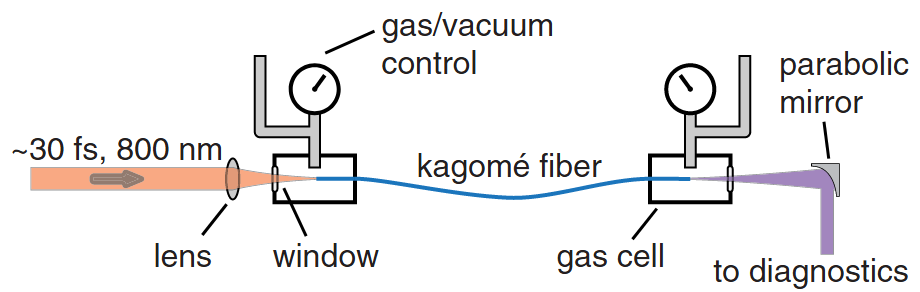
\includegraphics[width=0.4\textwidth]{p9.png}
    \caption{充气 Kagomé PCF 实验装置}\label{p3.1.1}
\end{figure}

本文提出的所有数值结果都是使用单向场传播方程计算的, 包括基于方程的全色散曲线、克尔效应、光电离以及通过光电离产生的自由电子的影响. 

\subsection{色散和非线性的相互作用}

超快非线性动力学取决于色散和非线性之间复杂的相互作用. 在这里使用简化的包络方程来对充气 Kagomé PCF 讨论. 将导模设为线偏振, 广义非线性薛定谔方程 (GNLSE) 采用归一化形式：
\begin{equation}
    \begin{aligned}\partial_zU&=-i\frac{\mathbf{sgn}(\beta_2)}{2L_D}\partial_\tau^2U+\frac{\mathbf{sgn}(\beta_3)}{6L_D^{\prime}}\partial_\tau^3U\\&+\frac{ie^{-az}}{L_{\mathbf{NL}}}(U|U|^2+is\partial_\tau(U|U|^2))\end{aligned}
    \label{eq:3.1.1}
\end{equation}
其中 $U(\tau,z)$ 是归一化光场包络, $\alpha$ 是损耗系数. 此处不存在拉曼效应, 尽管 $\beta_{4}$ 及更高阶色散可发挥重要作用, 但其不改变本节结果. 

$\tau_{0}$ 为泵浦脉冲持续时间, $\omega_{0}$ 为中心角频率, $P_{0}$ 为峰值功率, 以下归一化参数完整描述了传播动力学：
\begin{equation}
    \begin{aligned}&L_D=\frac{\tau_0^2}{|\beta_2|},\quad\quad L_D^{\prime}=\frac{\tau_0^3}{|\beta_3|},\\&\beta_n=\partial_\omega^n\beta|_{\omega_0},\quad\quad L_{\mathrm{NL}}=\frac1{\gamma P_0},\quad\quad s=\frac1{\omega_0\tau_0}\end{aligned}
    \label{eq:3.1.2}
\end{equation}

不失一般性, 假设泵浦脉冲以 800 nm 传播, 半峰全宽 (FWHM) 为 30 fs. 方程中\ref{eq:3.1.2}的长度尺度可简化为仅两个参数——ZDW $\lambda_{0}$ 和孤子阶数 N：
\begin{equation}
    (L_D,L_D^{\prime})\to\lambda_0\quad\quad(L_D,L_{\mathrm{NL}})\to N=\sqrt{\frac{\gamma P_0\tau_0^2}{|\beta_2|}}
    \label{eq:3.1.3}
\end{equation}

请注意, 虽然亮的孤子仅出现在反常色散区域, 但孤子阶次的定义也可用于正常色散区域, 以提供一种比较所有情况下相对非线性的便捷方法. 

将完整参数空间缩减为 ($\lambda_{0}$, N) 对于提取全局动态和理解给定系统的缩放行为非常有用. 例如, 若已知 $\lambda_{0}= 600\; \mathrm{nm}$ 和 N = 9 会导致 UV 产生, 则核心直径、气体种类、填充压力和脉冲能量的任意组合产生相同的值($\lambda_{0}$, N)也可以预期产生 UV. 请注意, 单独比较 $\lambda_{0}= 600\; \mathrm{nm}$ 或 N 是没有意义. 例如, 尽管几乎抽空的毛细管光纤将表现出远低于 200 nm 的反常色散, 但其非线性系数接近于零. 

\subsection{孤子的能量缩放：对色散情形的依赖}

通过再次考虑图 \ref{p2.0.4}, 可以充分理解 kagomé PCF 系统非凡的可扩展性. 对给定 ($\lambda_{0}$, N) , 可选择一种气体种类, 以及多种 kagomé PCF 直径选择, 找到适当压力固定 $\lambda_{0}$. 然后, 只需选择正确的脉冲能量即可得到给定孤子阶数 N. 

\begin{figure}[h]
    \centering
    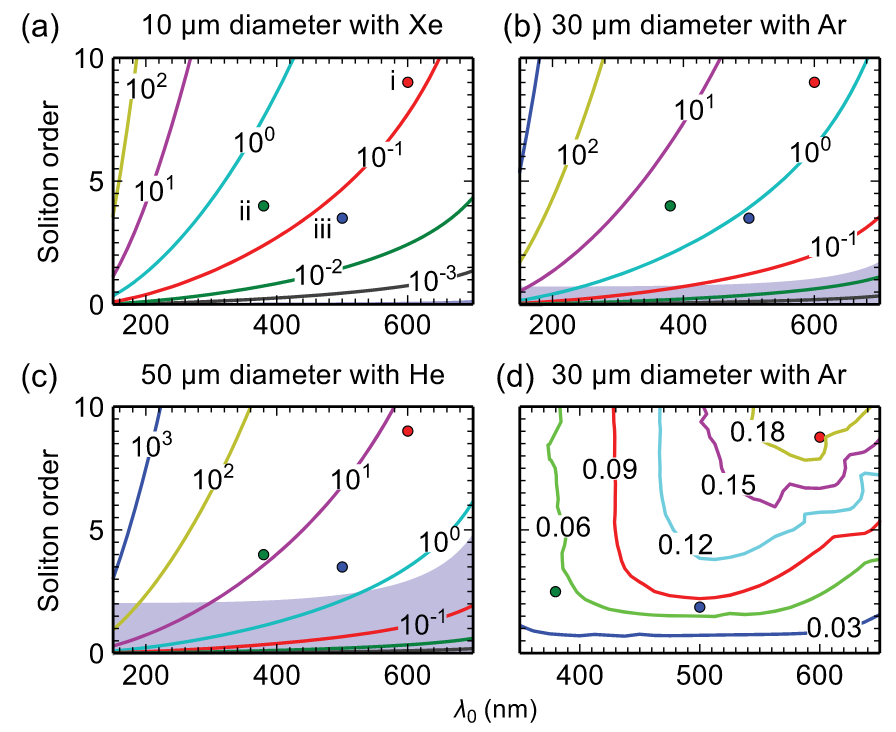
\includegraphics[width=0.4\textwidth]{p10.png}
    \caption{(a)–(c) 800 nm 处形成 30 fs 孤子所需的泵浦能量 ($\mathrm{\mu J}$) 的等值线图, 根据孤子级数和 ZDW 绘制, ZDW 通过改变气体压力进行调整：(a) 10 $\mathrm{\mu m}$ 直径充 Xe, (b) 直径 30 $\mathrm{\mu m}$, 充 Ar, (c) 直径 50 $\mathrm{\mu m}$, 充 He. 毛细管光纤中的整个参数空间将受到严重的损耗限制. 蓝色区域（下部阴影区域）是 kagomé PCF 的估计损失将限制非线性相互作用的地方.  (d) 在 kagomé PCF（芯直径 30 $\mathrm{\mu m}$, 充 Ar）中传播脉冲的峰值功率与临界自聚焦功率之比的等高线图, 根据孤子阶数和 ZDW 绘制, 包括脉冲自压缩效应. 标记点对应表 1 定义的系统. }\label{p3.2.1}
\end{figure}

图 7(a)-7(c) 显示了某些选定气体种类和 kagomé PCF 直径给定 ($\lambda_{0}$, N) 所需的能量范围. 

对于孤子阶数 $2 \leq N \leq 15$, 当在反常色散区域泵浦时, 传播动力学通常由孤子裂变主导, 这大致发生在特征长度尺度上：
\begin{equation}
    L_\mathrm{fiss}=\frac{L_D}N
    \label{eq:3.2.1}
\end{equation}

如果在此长度范围内功率损耗太高, 非线性传播将受限制（这里在一个孤子裂变长度上采用 1 dB 的指导值）. 对于毛细管纤维, 图 \ref{p3.2.1} (a)和 (b) 所呈现的所有三种情况下的整个参数空间上的非线性相互作用将被禁止. 尽管毛细管损耗随芯直径增大而减小, 但伴随非线性相互作用长度的增加抵消了这一点（由于较低的色散和较低的非线性）. 这意味着下面讨论的所有动力学都无法在毛细管纤维中实现. 相反, 图中的大部分参数空间可从 kagomé PCF 获取. 

从第 2.3 节讨论可看出, 对于图 \ref{p3.2.1} 中某些参数集, 所需能量可能太高. 即便如此至少一个系统可以访问所有动态, 而不会超过损坏阈值. 例如, 需要约 1 mJ 的能量才能在纤芯直径为 50 $\mathrm{\mu m}$、充 He 的 kagomé PCF 中产生八阶孤子, 从而产生 250 nm 的 ZDW. 如此高的脉冲能量可能超出了 Kagomé PCF 的处理能力；然而如果直径减小到 10 $\mathrm{\mu m}$, 用 Xe, 并且脉冲能量降低到 10 $\mathrm{\mu J}$（在 kagomé PCF 的能力范围内）, 也会产生相同的动力学结果. 

\begin{figure}[h]
    \centering
    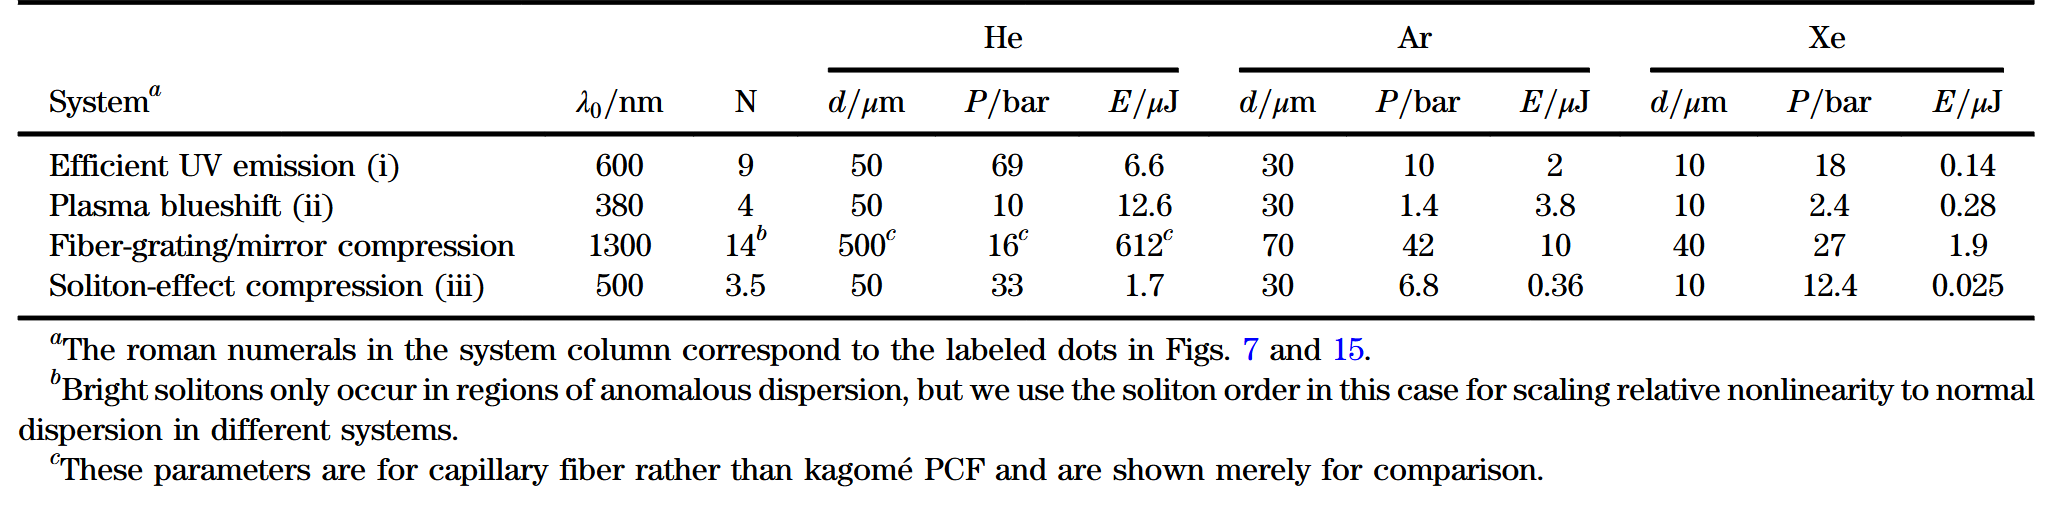
\includegraphics[width=1\textwidth]{p11.png}
    \caption{参数示例}\label{p3.2.2}
\end{figure}

一个更困难的问题是, 克尔效应引起的自聚焦或自由电子产生引起的散焦是否会显着干扰模式. 在大口径毛细管下, 泄漏模式的空间扰动发生在类似于散装气体中临界自聚焦所需的功率水平. 尽管在图 \ref{p3.2.1} 中的每种情况下发射的脉冲峰值功率都低于该限制, 但脉冲在传播时可能经历强烈的时间压缩. 为了量化这一点, 图 \ref{p3.2.1}(d) 绘制了自压缩后的峰值功率与相关气体压力下的临界自聚焦功率的比率. 对于 $\lambda_{0}= 600\;\mathrm{nm} $ 和 $N = 9$, 该比率达到最大值 $\sim$0.2, 这大约是N. Joly工作\cite{jolyBrightSpatiallyCoherent2011}中使用的参数, 其中没有观察到模式质量的下降. 这可能归因于峰值自压缩强度只能维持在太短的距离内, 自聚焦无法产生任何效果. 

一些参数示例总结如表格[图\ref{p3.2.2}].




%--------------------  插入参考文献  --------------------%

\newpage

\clearpage           %%%  “目录”中显示的页码正确, 需要添加 \clearpage
\phantomsection      %%   “目录”中的链接能正确跳转, 需要添加 \phantomsection
\addcontentsline{toc}{section}{参考文献}   %向目录中添加条目, 以章的名义

\bibliography{ref}

\end{document}